The Virtual Lab Assistant project aims to provide a comprehensive digital platform for conducting, managing, and evaluating practical examinations in a virtual environment. Traditional manual systems of practical exams often involve significant logistical challenges, such as limited lab resources, scheduling conflicts, and inconsistent evaluation methods. The Virtual Lab Assistant system overcomes these issues by creating a real-time, interactive, and secure online environment where students can perform their practical tasks efficiently under supervised conditions.
This chapter presents a detailed introduction to the project, including its background, motivation, problem definition, scope, objectives, and the chosen software development model. 


The organization of this chapter is as follows: Section 1.1 discusses the background, motivation described in Section 1.2. Section 1.3 defines the problem statement, the scope is explained in Section 1.4. Section 1.5 lists the objectives, the life cycle model explained in Section 1.6.
Section 1.7 describes the report organization, Section 1.8 summarizes the chapter.

 



\section{Background}

With the rapid digital transformation in education, traditional methods of conducting practical exams are being replaced by virtual and automated solutions. Manual evaluation, scheduling, and monitoring of practical exams often result in inefficiencies and delays. The Virtual Lab Assistant system introduces a digital platform that simulates real laboratory conditions where students can log in, attempt practical assignments, compile and execute code, and receive instant feedback.

\section{Motivation}
The main motivation behind developing the Virtual Lab Assistant is to modernize the process of conducting and evaluating practical examinations in academic institutions.
In many colleges and universities, students face difficulties during lab exams due to time constraints, unavailability of systems, and manual evaluation delays. Similarly, instructors spend a significant amount of time organizing, supervising, and assessing practical submissions.
By introducing a virtual and secure platform, the Virtual Lab Assistant aims to:
•	Enhance accessibility for students to perform practicals from any location.
•	Automate the evaluation process using integrated compilers and real-time feedback.
•	Reduce administrative effort and ensure consistent grading standards.

This system promotes digital learning, supports remote education, and aligns with the vision of a smart education ecosystem.


\section{Problem Definition}
Existing systems for practical examinations suffer from numerous drawbacks:
\item •	Manual scheduling leads to confusion and overlap of exam slots.
\item •	Lack of centralized evaluation increases subjectivity and delays in results.
\item •	Limited supervision and monitoring allow for unfair means during exams.
\item •	Difficulty in maintaining performance records and analytics for each student.



\section{Scope}
The scope of the Virtual Lab Assistant includes:
The scope of the Virtual Lab Assistant project is to provide a web-based platform for conducting DBMS practical exams where students can log in, attempt SQL queries, and receive basic syntax-based evaluation. It allows admin to monitor student participation, manage exams, and view performance based on correct answers and percentage results. The system ensures a controlled environment with login restrictions and timed exams. However, the project is limited to basic SQL validation and does not execute queries on a real database. It also supports limited subjects and lacks advanced security or real-time proctoring features.

Future enhancements may include voice-based assistance, AI-based evaluation of code, and integration with institutional databases.



\section{Objective}
The primary objectives of the Virtual Lab Assistant are:
\item 1.	To develop a secure and efficient online platform for conducting practical examinations.
\item 2.	To integrate automatic code compilation and evaluation systems.
\item 3.	To enable the administrator to manage questions, exam dates, and subjects dynamically.


\section{Selection Of Life Cycle Model}                                                                                                                           The Waterfall Model is selected for developing the Virtual Lab Assistant.
It is a linear and sequential approach where each phase of the development process flows downward to the next, like a waterfall. This model is most suitable when requirements are well-defined and do not change frequently.
The Figure 1.1 shows Selection Of Life Cycle Model (Prototype Model).


\begin{figure}[H]
    %\begin{center}
    \centering
    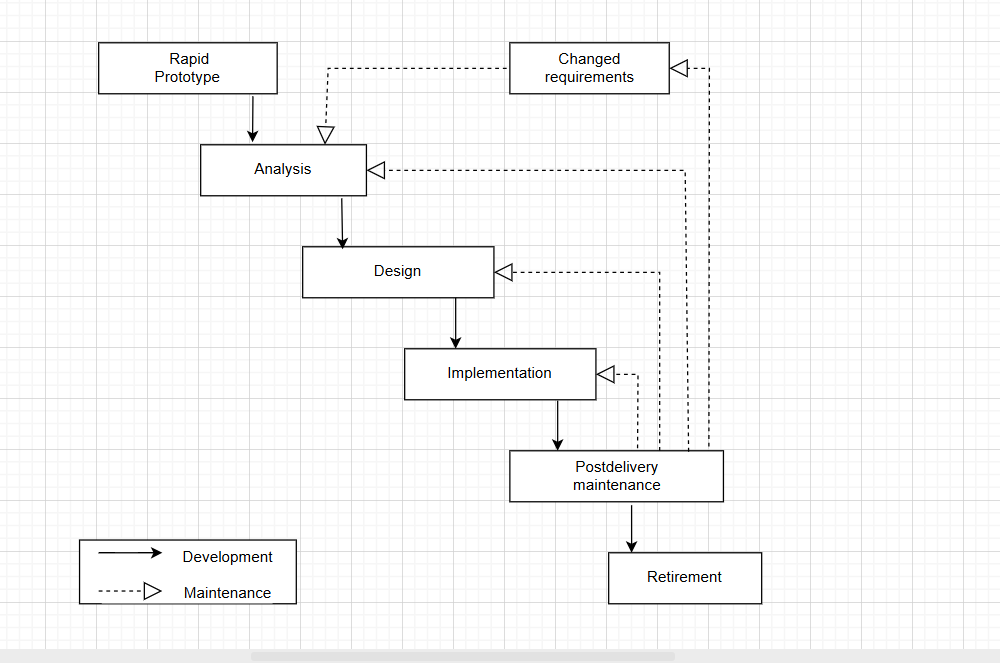
\includegraphics[width=15cm, height=7cm]{chapters/Prototype new.png}
    \caption{Selection Of Life Cycle Model (Prototype Model}
    
    %\vspace{-0.3cm}
\end{figure}

Waterfall Model  is best suited model for this project:
\begin{enumerate}
    \item 	The system requirements are clear and well-documented..
    \item 	The development process is straightforward, with distinct phases of analysis, design, implementation, testing, and deployment.

   \item Limited user participation is required during early stages, making it ideal for academic projects.
 
   \item Ensures timely completion of each phase before moving to the next.

\end{enumerate}


\section{Organization of Report}

The organization of the report is structured as follows:

\begin{itemize}

\item \textbf{CHAPTER 1} \\
Titled as \textbf{Introduction}, this chapter describes the background of the project, problem definition, scope and objectives, and the overall structure of the report.

\item \textbf{CHAPTER 2} \\
Titled as \textbf{Planning}, this chapter includes feasibility study, risk analysis, project scheduling, effort estimation, and cost estimation.

\item \textbf{CHAPTER 3} \\
Titled as \textbf{Analysis}, this chapter explains requirement collection and identification, hardware and software requirements, functional and non-functional requirements.

\item \textbf{CHAPTER 4} \\
Titled as \textbf{Design}, this chapter presents system architecture, data flow diagrams, database design, and UML diagrams.

\item \textbf{CHAPTER 5} \\
Titled as \textbf{Coding/Implementation}, this chapter describes the algorithms, development tools, technologies used, and different modules implemented in the system.

\item \textbf{CHAPTER 6} \\
Titled as \textbf{Testing}, this chapter includes testing methodologies such as black box and white box testing, manual and automated testing, and test case identification and execution.

\item \textbf{CHAPTER 7} \\
Titled as \textbf{Results and Discussion}, this chapter presents the output of the system, performance analysis, and discussion of the results obtained.

\item \textbf{CHAPTER 8} \\
Titled as \textbf{Conclusion and Future Work}, this chapter summarizes the overall project outcomes and suggests possible future enhancements.

\end{itemize}





\end{itemize}

\section{Summary}
 In this Chapter, Introduction is presented. In the next Chapter, Project Planning And Management is discussed.


